% Avsluttende prosjekt i INF5620

\documentclass[a4paper, 10pt]{article}
\usepackage[utf8x]{inputenc}
\usepackage{cancel}
\usepackage{graphicx}
\newcommand{\mb}{\mathbf}
\newcommand{\mc}{\mathcal}
\newcommand{\n}{\nabla}

\author{Henrik Andersen Sveinsson}
\title{Avsluttende prosjekt - INF5620}

\begin{document}
\maketitle

Prosjektet går ut på å løse den ikke-lineære diffusjonslikningen: 

\begin{equation}
	\rho u_t = \nabla \cdot (\alpha(u) \nabla u) + f(\mb{x}, t)
\end{equation}

med initialbetingelse:
\begin{equation}
	u(\mb{x}, 0) = I(\mb{x})
\end{equation}


og Neumannbetingelse:
\begin{equation}
	\frac{\partial u}{\partial n} = 0
\end{equation}

\section{Tidsdiskretisering}
Bruker backward Euler på den tidsderiverte:

\begin{equation}
	\rho \frac{u - u_1}{\Delta t} = \n \cdot (\alpha(u) \n u) + f(\mb{x}, t)
\end{equation}
\begin{equation}
	\rho u - \Delta t\n \cdot (\alpha(u) \n u) = \rho u_1 + \Delta t f(\mb{x}, t)
\end{equation}

Den variasjonelle formuleringen for det romlige problemet i hvert tidssteg blir:

\begin{equation}
	\rho (u, v) - \Delta t \left[ (\alpha(u) \nabla u, \nabla v) + \cancel{\left( \alpha(u) \frac{\partial u}{\partial n}, v\right)_{\partial \Omega}}\right] = \rho(u_1, v) + \Delta t (f, v)
\end{equation}

Der Neumannbetingelsen eliminerer grenseflateintegralet. 
Merk at i den siste likningen er $u = \sum c_j \psi_j$, og likningen setter residualet ortogonalt på løsningen i den opprinnelige likningen. 

\subsection{Variasjonell formulering av initialbetingelsen}
\begin{equation}
	u_e(\mb{x}, 0) \approx u(\mb{x}, 0) =  \sum c_j \psi_j
\end{equation}

Setter:
\begin{equation}
	R = u(\mb{x}, 0)-I(\mb{x})
\end{equation}
Krever at:
\begin{equation}
	\int_{\Omega} Rv = 0
\end{equation}
Altså at:
\begin{equation}
	(u, v) = (I, v)
\end{equation}
Med elementfunksjoner får vi at initialbetingelsen blir:
\begin{equation}
	u(\mb{x}, 0) = \sum I(\mb{x}_{\nu(j)}) \varphi_{\nu(j)}
\end{equation}

\section{Picard-iterasjon}
Lineariserer den variasjonelle formuleringen for å kunne anvende Picard-iterasjon.

\begin{equation}
	\rho(u, v) - \Delta t (\alpha(u\_)\nabla u, \nabla v) = \rho(u_1,v) + \Delta t (f, v)
\end{equation}
Setter så inn at $v$ er alle $\psi$ i et eller annet rom, som er det samme rommet som vi ekspanderer $u$ i. 
\begin{equation}
\sum_{j \in \mc{I}_s} \left[\rho(\psi_j, \psi_i) - \Delta t (\alpha(u\_)\nabla\psi_j, \nabla\psi_i) \right]c_j	
= \rho(u\_, \psi_i)+  \Delta t (f, \psi_i) \ \ \forall \ \ i
\end{equation}
Picard-iterasjon på denne, vil si å løse dette likningssettet med hensyn på $u = \sum c_j \psi_j$, og oppdatere $u\_$. 

\section{Implementasjon}
Tidsintegrasjon med 1-stegs picarditerasjon er implementert. E/h er konstant (vist ved testing for varierende oppløsning).

\section{Manufactured solution}
Likningen skal løses i 1D på $\Omega = [0, 1]$. Den ikke-lineære faktoren er $\alpha = 1 + u^2$ og løsningen skal være:
\begin{equation}
	u(x,t) = t\int_0^x q(1-q)dq = tx^2\left(\frac{1}{2} - \frac{x}{3}\right)
\end{equation}

Med sympy vises det da at kildeleddet f skal være:
\begin{equation}
	f(x, t) = - \frac{1}{3} \rho x^{3} + \frac{1}{2} \rho x^{2} + \frac{8}{9} t^{3} x^{7} - \frac{28}{9} t^{3} x^{6} + \frac{7}{2} t^{3} x^{5} - \frac{5}{4} t^{3} x^{4} + 2 t x - t
\end{equation}

Forskjellen mellom løsningen her og løsningen i FEniCS bør være av orden $\Delta t$, siden jeg bruker et Backward Euler skjema. 

Innsetting av dette i den numeriske metoden gir en feil som går som $/Delta t$, som vist i figur \ref{fig:convergence_manufactured_1d}.

\begin{figure}
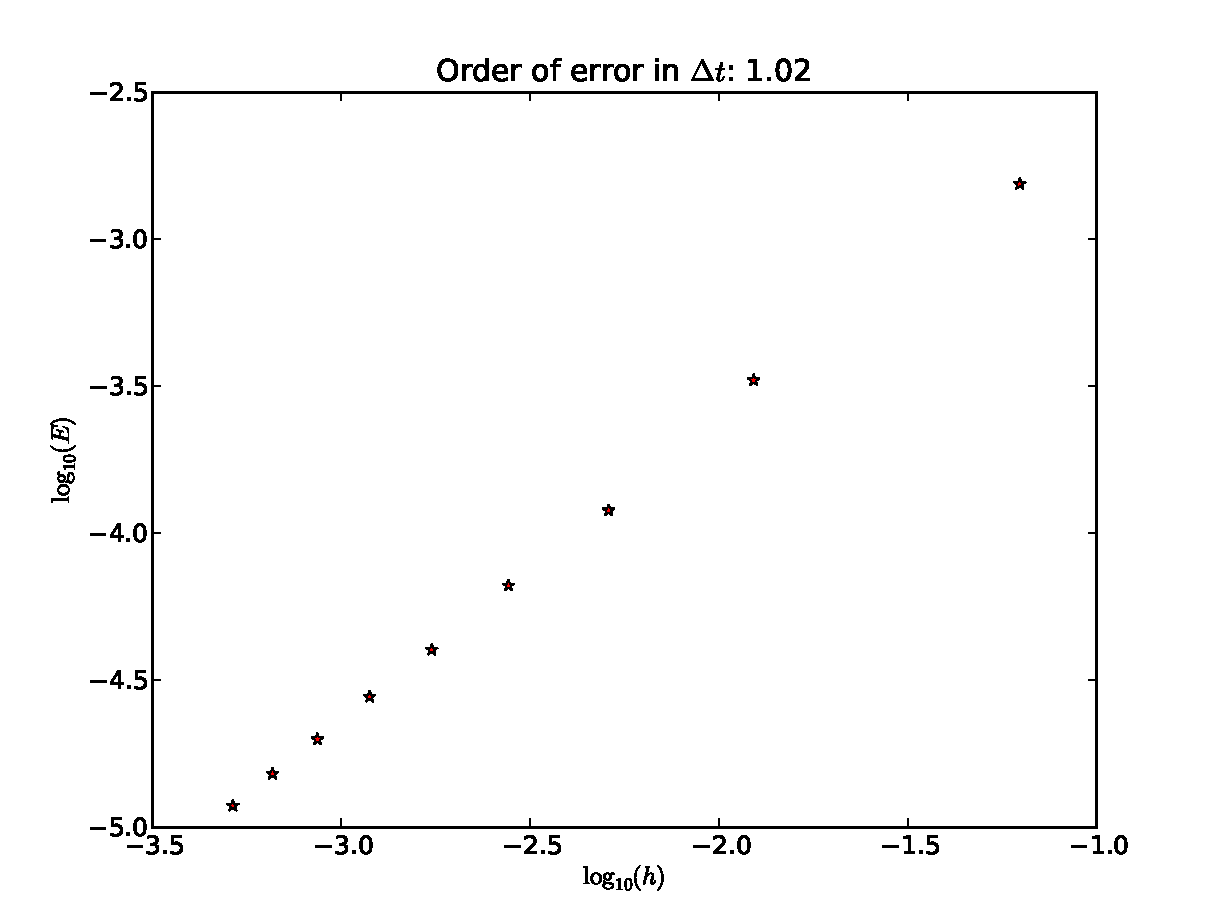
\includegraphics[width=\textwidth]{figures/convergence_manufactured_1d.pdf}
\caption{Figuren viser at feilen med \emph{manufactured solution} nesten er i orden $\Delta t$.}
\label{fig:convergence_manufactured_1d}.
\end{figure}

\end{document}